\section{Breath-First and Depth-First Search}
\subsection{High-Level Overview}
Two general methods for traversing a graph are, \textbf{breadth-first search} and \textbf{depth-first search}.

\label{sec:bfs_dfs}
\begin{Def}[Cycle]

    A \textbf{cycle} is a path that starts and ends at the same node.
\end{Def}
\textbf{Example:} In the above Figure (\ref{fig:adj_matri_dir}), $1\rightarrow 2 \rightarrow 3 \rightarrow 1$ form a cycle.
\begin{Def}[Tree]

    A \textbf{tree} is a connected graph with no cycles. A \textbf{leaf-nodes} is the outer-most nodes of a tree. A \textbf{branch} is a path from the root to a leaf.  
\end{Def}
\newpage
\begin{theo}[Tree Identity]

    Let $G$ be an undirected graph of $n$ nodes. Then any two statements imply the third:
    \begin{enumerate}
        \item [(i.)] $G$ is connected.
        \item [(ii.)] $G$ has $n-1$ edges.
        \item [(iii.)] $G$ has no cycles.
    \end{enumerate}
\end{theo}

\begin{Def}[Rooted Trees]
    
        Let $T$ be a tree with a designated root node $r$. Then each degree is 
        considered an outdegree, called a \textbf{child}, and its indegree its \textbf{parent}.
\end{Def}
\begin{figure}[h]
    \begin{center}
      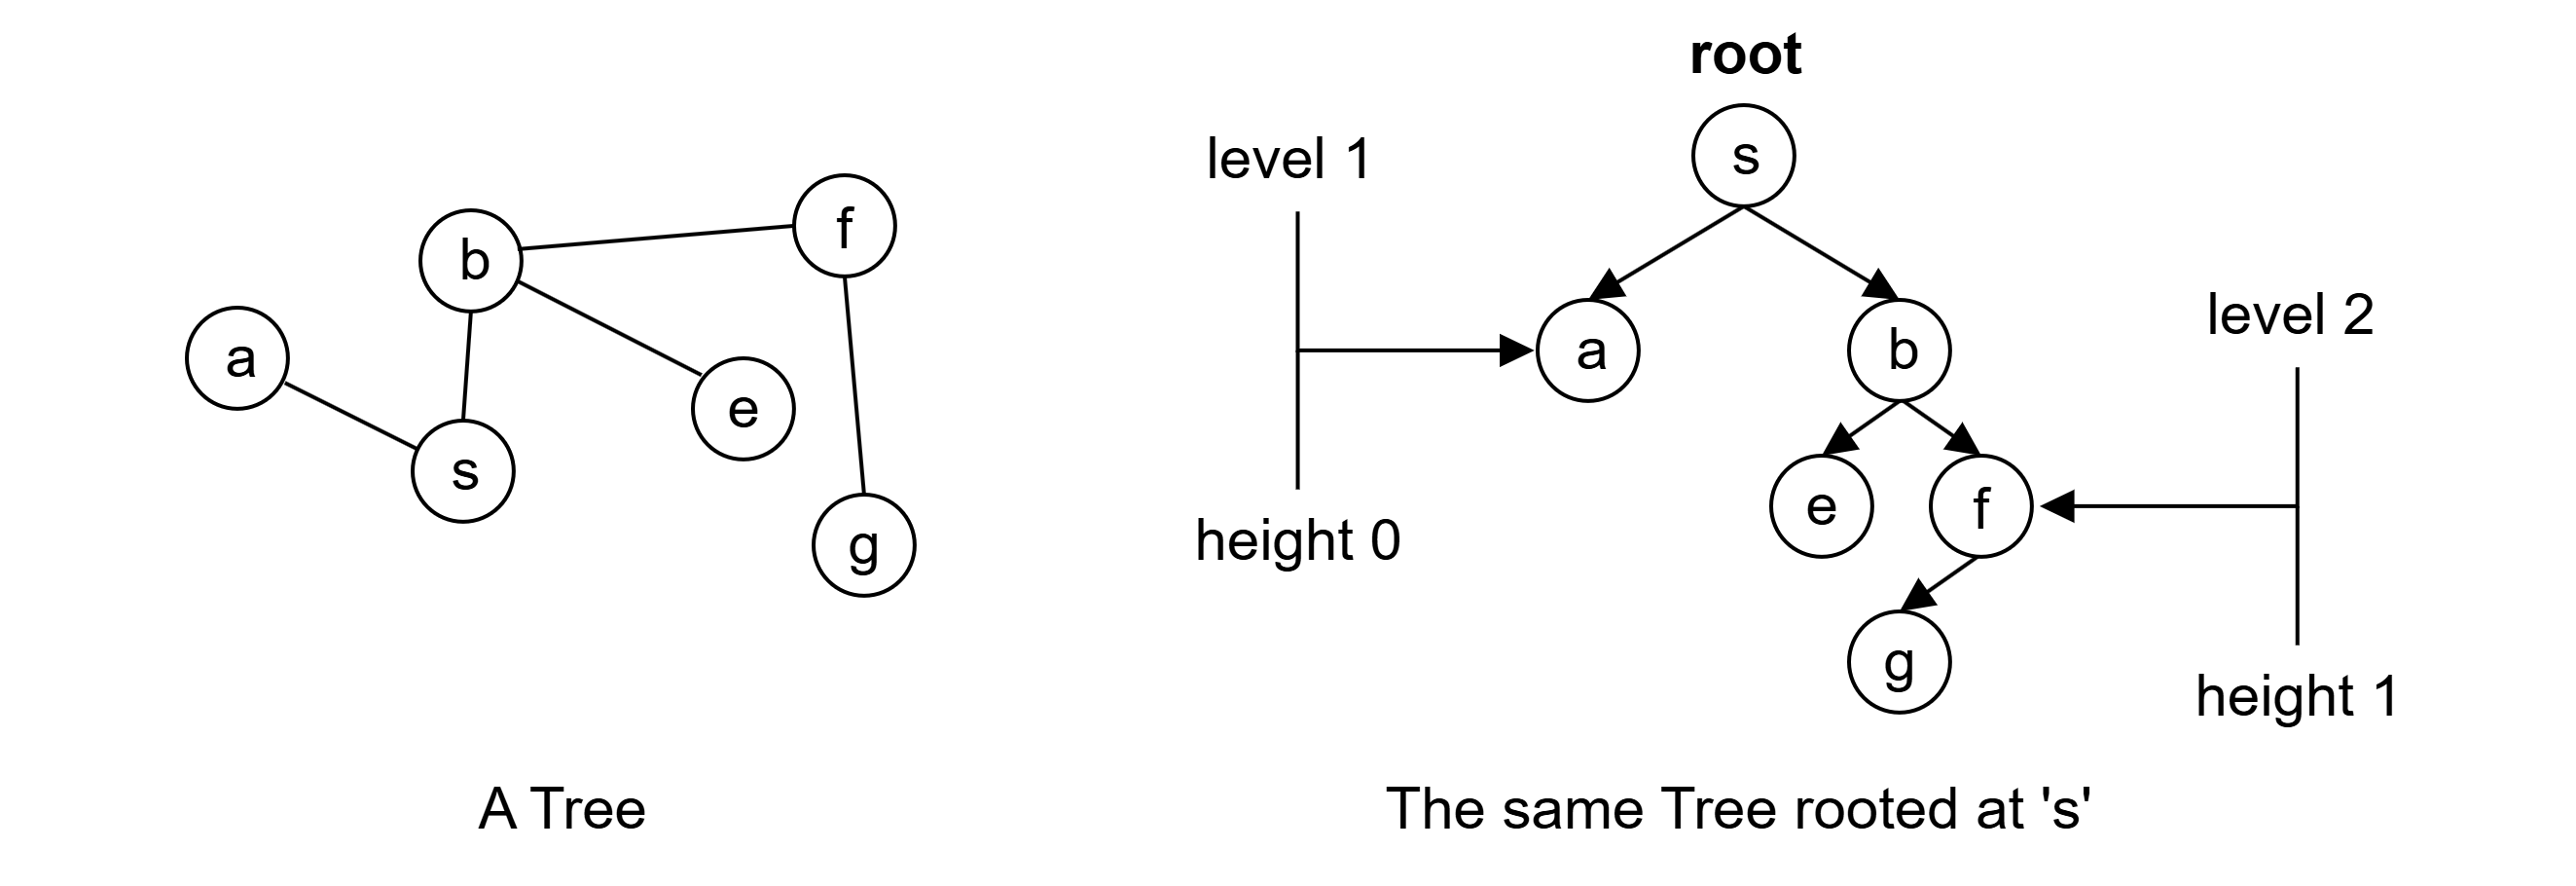
\includegraphics[height=2in]{./Sections/graphs/rooted_tree.png}
    \end{center}
     \caption{A rooted tree with root 1 and children $\{2,5,7\}$}\label{fig:rooted_tree}
  \end{figure}

\begin{Def}[Levels and Heights]

    The \textbf{level} of a node is the number of edges from the root. The \textbf{height} of a tree is the maximum level of any node.
\end{Def}
\textbf{Example:} In Figure (\ref{fig:rooted_tree})'s rooted tree , node 5 has a level of 1, and the height of the tree is 2.
\newpage
\begin{Def}[Breadth-First Search (BFS)]

    In a \textbf{breadth-first search}, we start at a node's children first before moving onto their children's children in level order.
\end{Def}
\begin{figure}[h]
    \begin{center}
      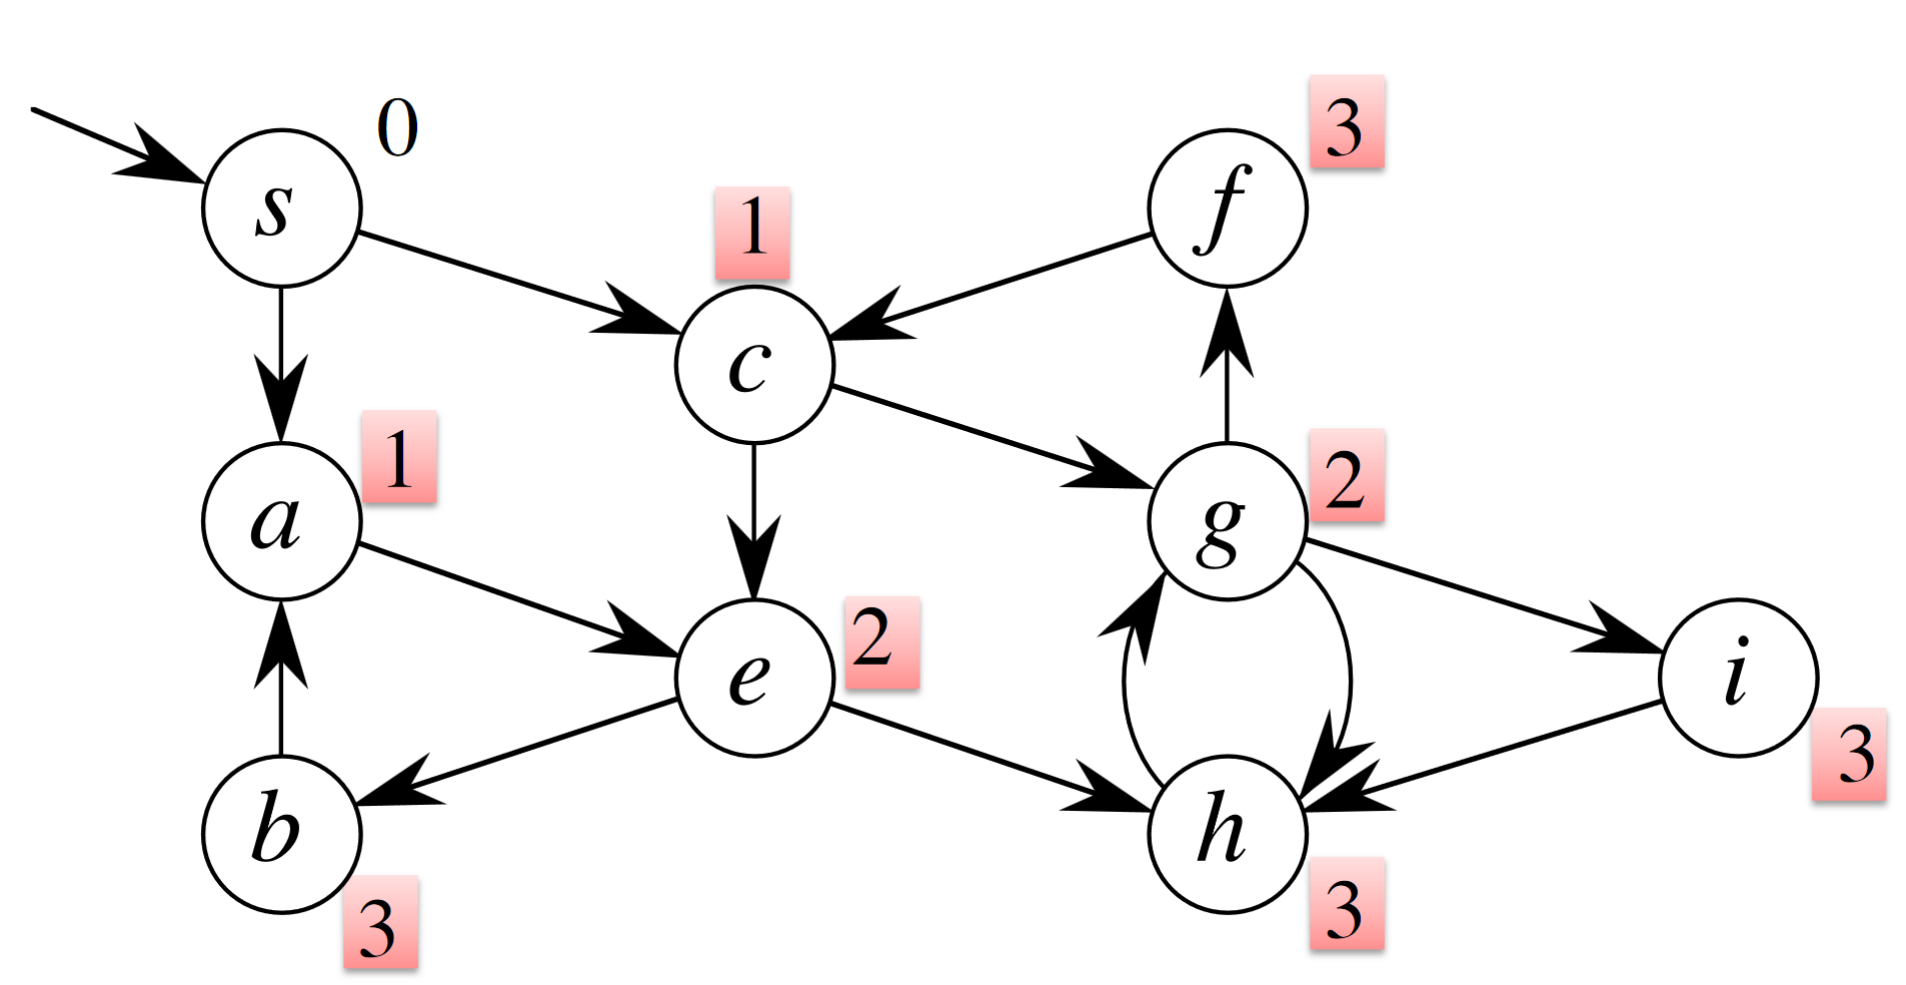
\includegraphics[height=2in]{./Sections/graphs/bfs.png}
    \end{center}
     \caption{A BFS tree traversal preformed on a graph with each level enumerated}\label{fig:bfs}
  \end{figure}

\begin{theo}[Properties of BFS]
    
    BFS run on any graph $T$ produces a tree $T'$ with the following properties:
    \begin{enumerate}
        \item [(i.)] $T'$ is a tree.
        \item [(ii.)] $T'$ is a rooted tree with the starting node as the root.
        \item [(iii.)] The height of $T'$ is the shortest path from the root to any node.
        \item [(iv.)] Any sub-paths of $T'$ are also shortest paths.
    \end{enumerate}
\end{theo}
\begin{Proof}[Proof of BFS]

    (i.) and (ii.) follow from the definition of a tree. (iii.) and (iv.) follow that since a tree 
    contains a direct path to any given node in our parent child relationship, that path must be the shortest.
\end{Proof}
\begin{Tip}
    In a family tree, there is only one path from each ancestor to each descendant.
\end{Tip}

\newpage 

\noindent
We create a BFS algorithm from what we know, though not the best implementation:
\begin{Func}[BFS Algorithm - \texttt{BFS($s$)}]
    Breadth-First Search starting from node $s$.
    
    \vspace{.5em}
    \noindent
    \textbf{Input:} Graph $G = (V, E)$ and starting node $s$.\\
    \textbf{Output:} Levels of each vertex from $s$.\\
    \begin{algorithm}[H]
        \SetAlgoLined
        \SetKwProg{Fn}{Function}{:}{}
        \Fn{\texttt{BFS($s$)}}{
            \For{each $v \in V$}{
                Level[$v$] $\gets \infty$\;
            }
            Level[$s$] $\gets 0$\;
            Add $s$ to $Q$\;
            \While{$Q$ not empty}{
                $u \gets Q$.Dequeue()\;
                \For{each $v \in G[u]$}{
                    \If{Level[$v$] $= \infty$}{
                        Add edge $(u, v)$ to tree $T$ (parent[$v$] $= u$)\;
                        Add $v$ to $Q$\;
                        Level[$v$] $\gets$ Level[$u$] + 1\;
                    }
                }
            }
        }
    \end{algorithm}
\end{Func}
\vspace{-2em}
\begin{figure}[h]
    \begin{center}
      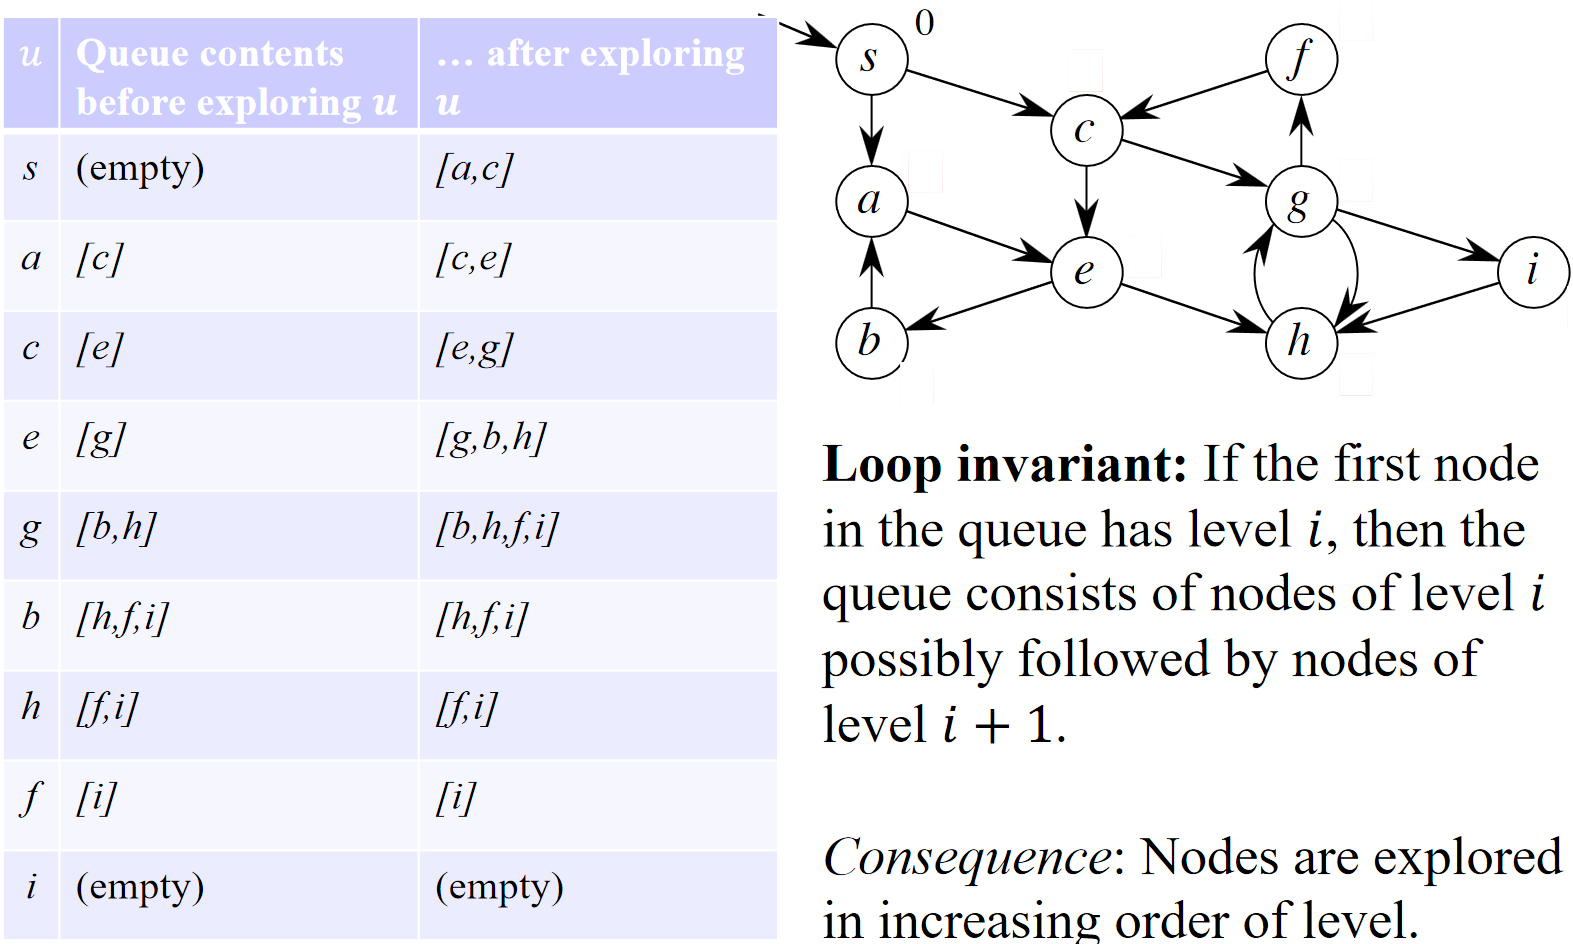
\includegraphics[height=2.9in]{./Sections/graphs/bfs_q.png}
    \end{center}
     \caption{A table showing the queue at each level of iteration}\label{fig:bfs_q}
  \end{figure}

  \newpage

We analyze the time and space complexity in the below Figure (\ref{fig:bfs_q_ana}):

\begin{figure}[h]
    \begin{center}
      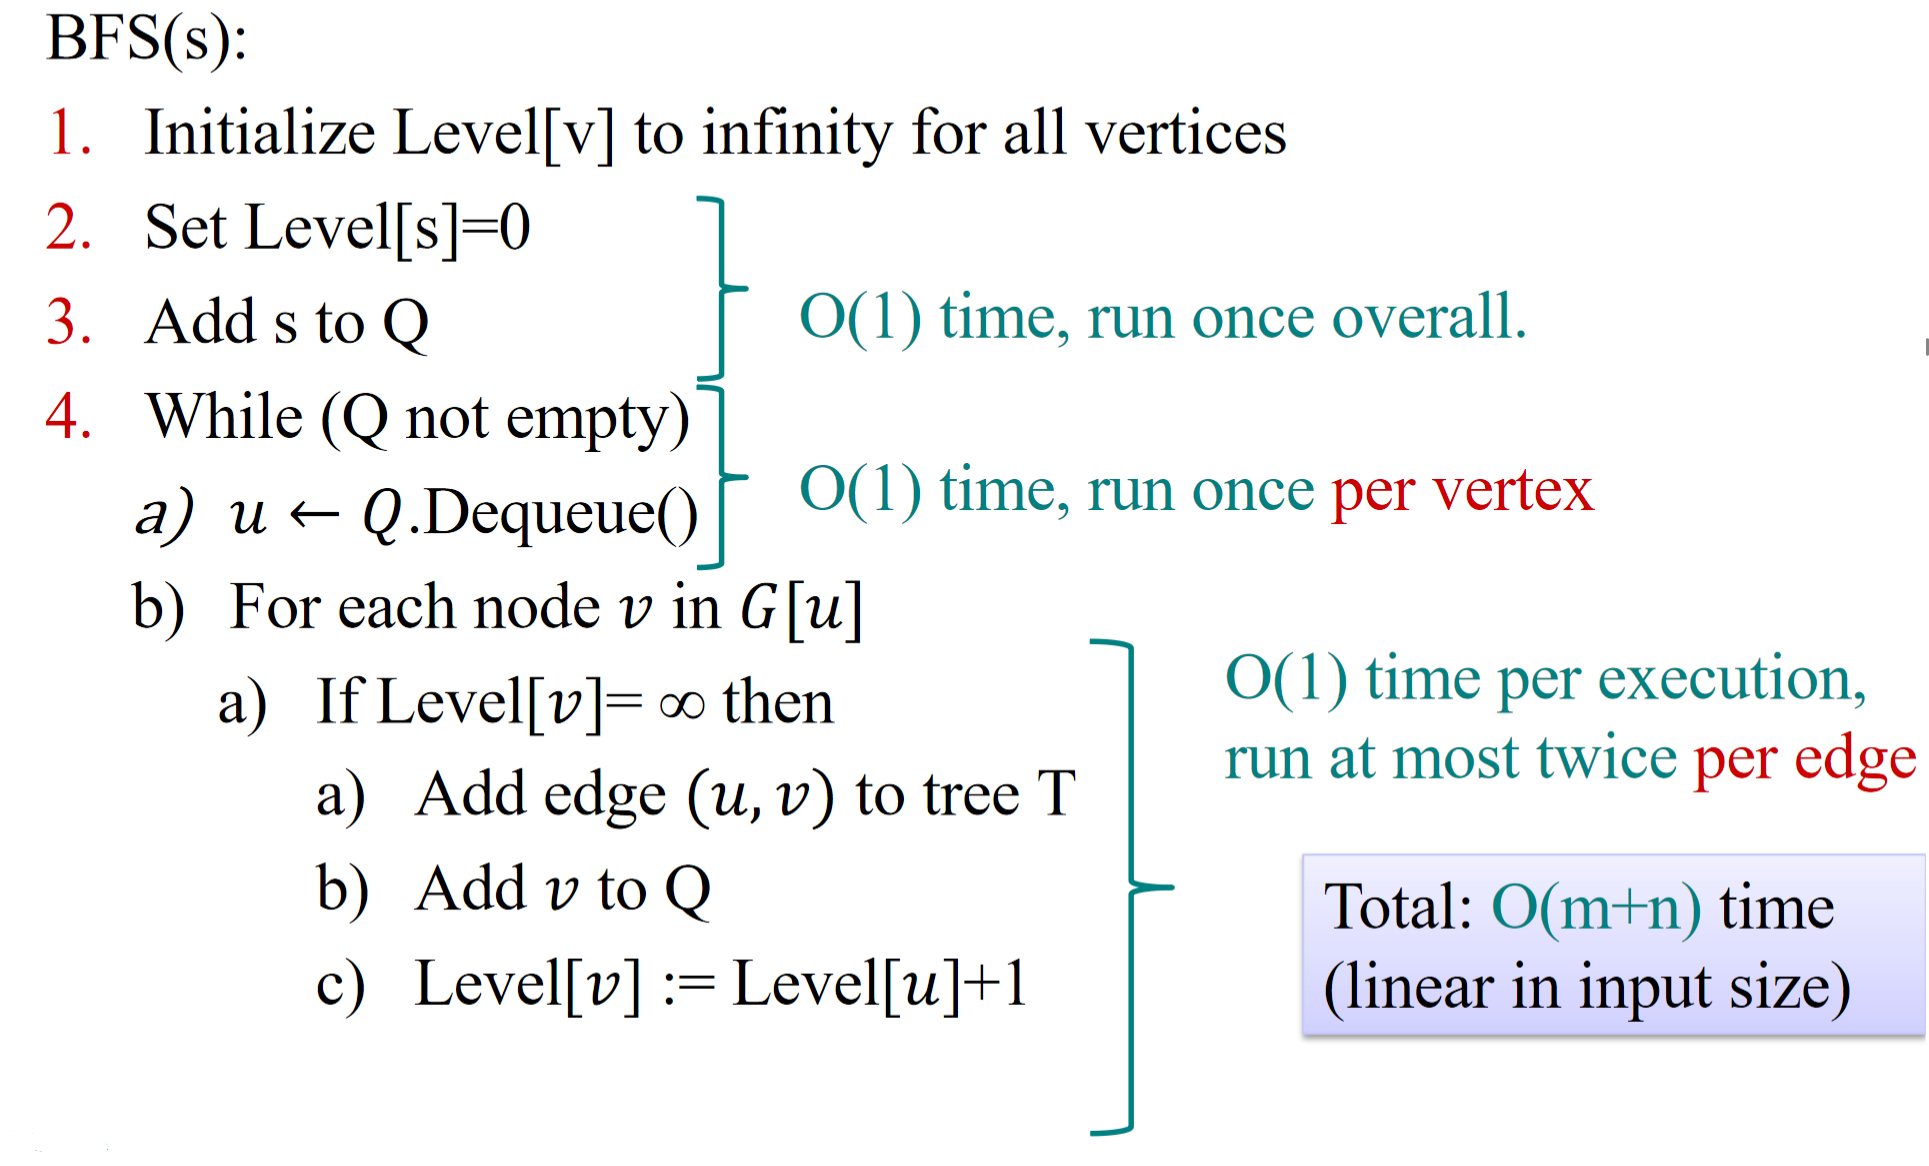
\includegraphics[height=2in]{./Sections/graphs/bfs_q_ana.png}
    \end{center}
     \caption{An analysis showing $O(m+n)$ for both time and space complexity}\label{fig:bfs_q_ana}
  \end{figure}
  \begin{Proof}[Claim 1 for BFS]
    Let $s$ be the root of the BFS tree, then:
    \textbf{Proof:} Induction on the distance from $s$ to $u$.\\
    \textbf{Base case} ($u = s$): The code sets Level[$s$] = 0, and there is no path to find since the path has length 0.\\
    \textbf{Induction hypothesis:} For every node $u$ at distance $\leq i$, Claim 1 holds.\\
    \textbf{Induction step:}
    \begin{itemize}
        \item Let $v$ be a node at distance exactly $i + 1$ from $s$. Let $u$ be its parent in the BFS tree.
        \item The code sets Level[$v$] = Level[$u$] + 1.
        \item Let $x$ be the last node before $v$ on a shortest path from $s$ to $v$. Since $v$ is at distance $i + 1$, then $x$ must be at distance $i$, and so Level[$x$] = $i$ (by induction hypothesis).
        \item If $u = x$, we are done!
        \item If $u \neq x$, then it must be that $u$ was explored before $x$, since otherwise $x$ would be the parent of $u$.
        \item Since we explore nodes in order of level, Level[$u$] $\leq$ Level[$x$] = $i$.
        \item If Level[$u$] = $i$, then we are done.
        \item If Level[$u$] $<$ $i$, then the path $s \sim u \to v$ has length at most $i$, which contradicts the assumption that the distance of $v$ is $i + 1$.
    \end{itemize}
    
    \noindent
    We conclude that Level[$u$] = $i$, Level[$v$] = $i + 1$, and the path in the BFS tree that goes from $s$ to $u$ to $v$ has length $i + 1$.
    \end{Proof}
    
    \newpage
    \begin{Def}[Depth-First Search (DFS)]

        In a \textbf{depth-first search}, we recursively explore each an entire branch before moving onto the next.
    \end{Def}

    \begin{Func}[DFS Algorithm - \texttt{DFS($G$)}]
        Depth-First Search on graph $G$ (recursive).
    
        \vspace{.5em}
        \noindent
        \textbf{Input:} Graph $G = (V, E)$.\\
        \textbf{Output:} Discovery and finishing times for each vertex.
        
        \begin{algorithm}[H]
            \SetAlgoLined
            \SetKwProg{Fn}{Function}{:}{}
            \Fn{\texttt{DFS($G$)}}{
                \For{each $u \in G$}{
                    $u$.state $\gets$ \texttt{unvisited}\;
                }
                time $\gets 0$\;
                \For{each $u \in G$}{
                    \If{$u$.state == \texttt{unvisited}}{
                        \texttt{DFS-Visit($u$)}\;
                    }
                }
            }
            \vspace{.5em}
            \Fn{\texttt{DFS-Visit($u$)}}{
                time $\gets$ time + 1\;
                $u.d \gets$ time \; // record discovery time\;
                $u$.state $\gets$ \texttt{discovered}\;
                \For{each $v \in G[u]$}{
                    \If{$v$.state == \texttt{unvisited}}{
                        \texttt{DFS-Visit($v$)}\;
                    }
                }
                $u$.state $\gets$ \texttt{finished}\;
                time $\gets$ time + 1\;
                $u.f \gets$ time\; // record finishing time\;
            }
        \end{algorithm}

        \noindent
        \textbf{Time and Space Complexity:} $O(n+m)$ where $n$ is the number of vertices and $m$ the number of edges.
    \end{Func}

    \newpage

    \begin{Proof}[DFS Correctness]

        \textbf{Case 1:} When $s$ is discovered, there is a path of unvisited vertices from $s$ to $y$. We use induction on the length $L$ of the unvisited path from $x$ to $y$.
        \begin{itemize}
            \item \textbf{Base case:} There is an edge $(x, y)$, and $y$ is unvisited.
            \item \textbf{Induction hypothesis:} Assume that the claim is true for all nodes reachable via $k$ unvisited nodes.
            \item \textbf{Induction step:}
            \begin{itemize}
                \item Consider $u$ reachable via $k + 1$ unvisited nodes.
                \item Let $z$ be the last node on the path before $y$, and $z$ is discovered from $x$ (by I.H.).
                \item The edge $(z, y)$ will be explored from $x$, ensuring that $y$ is eventually visited.
            \end{itemize}
        \end{itemize}
        \noindent
        Thus, DFS-Visit($x$) explores all nodes reachable from $x$ through a path of unvisited nodes, as required.
        \end{Proof}

% \begin{figure}[h]
%     \begin{center}
%       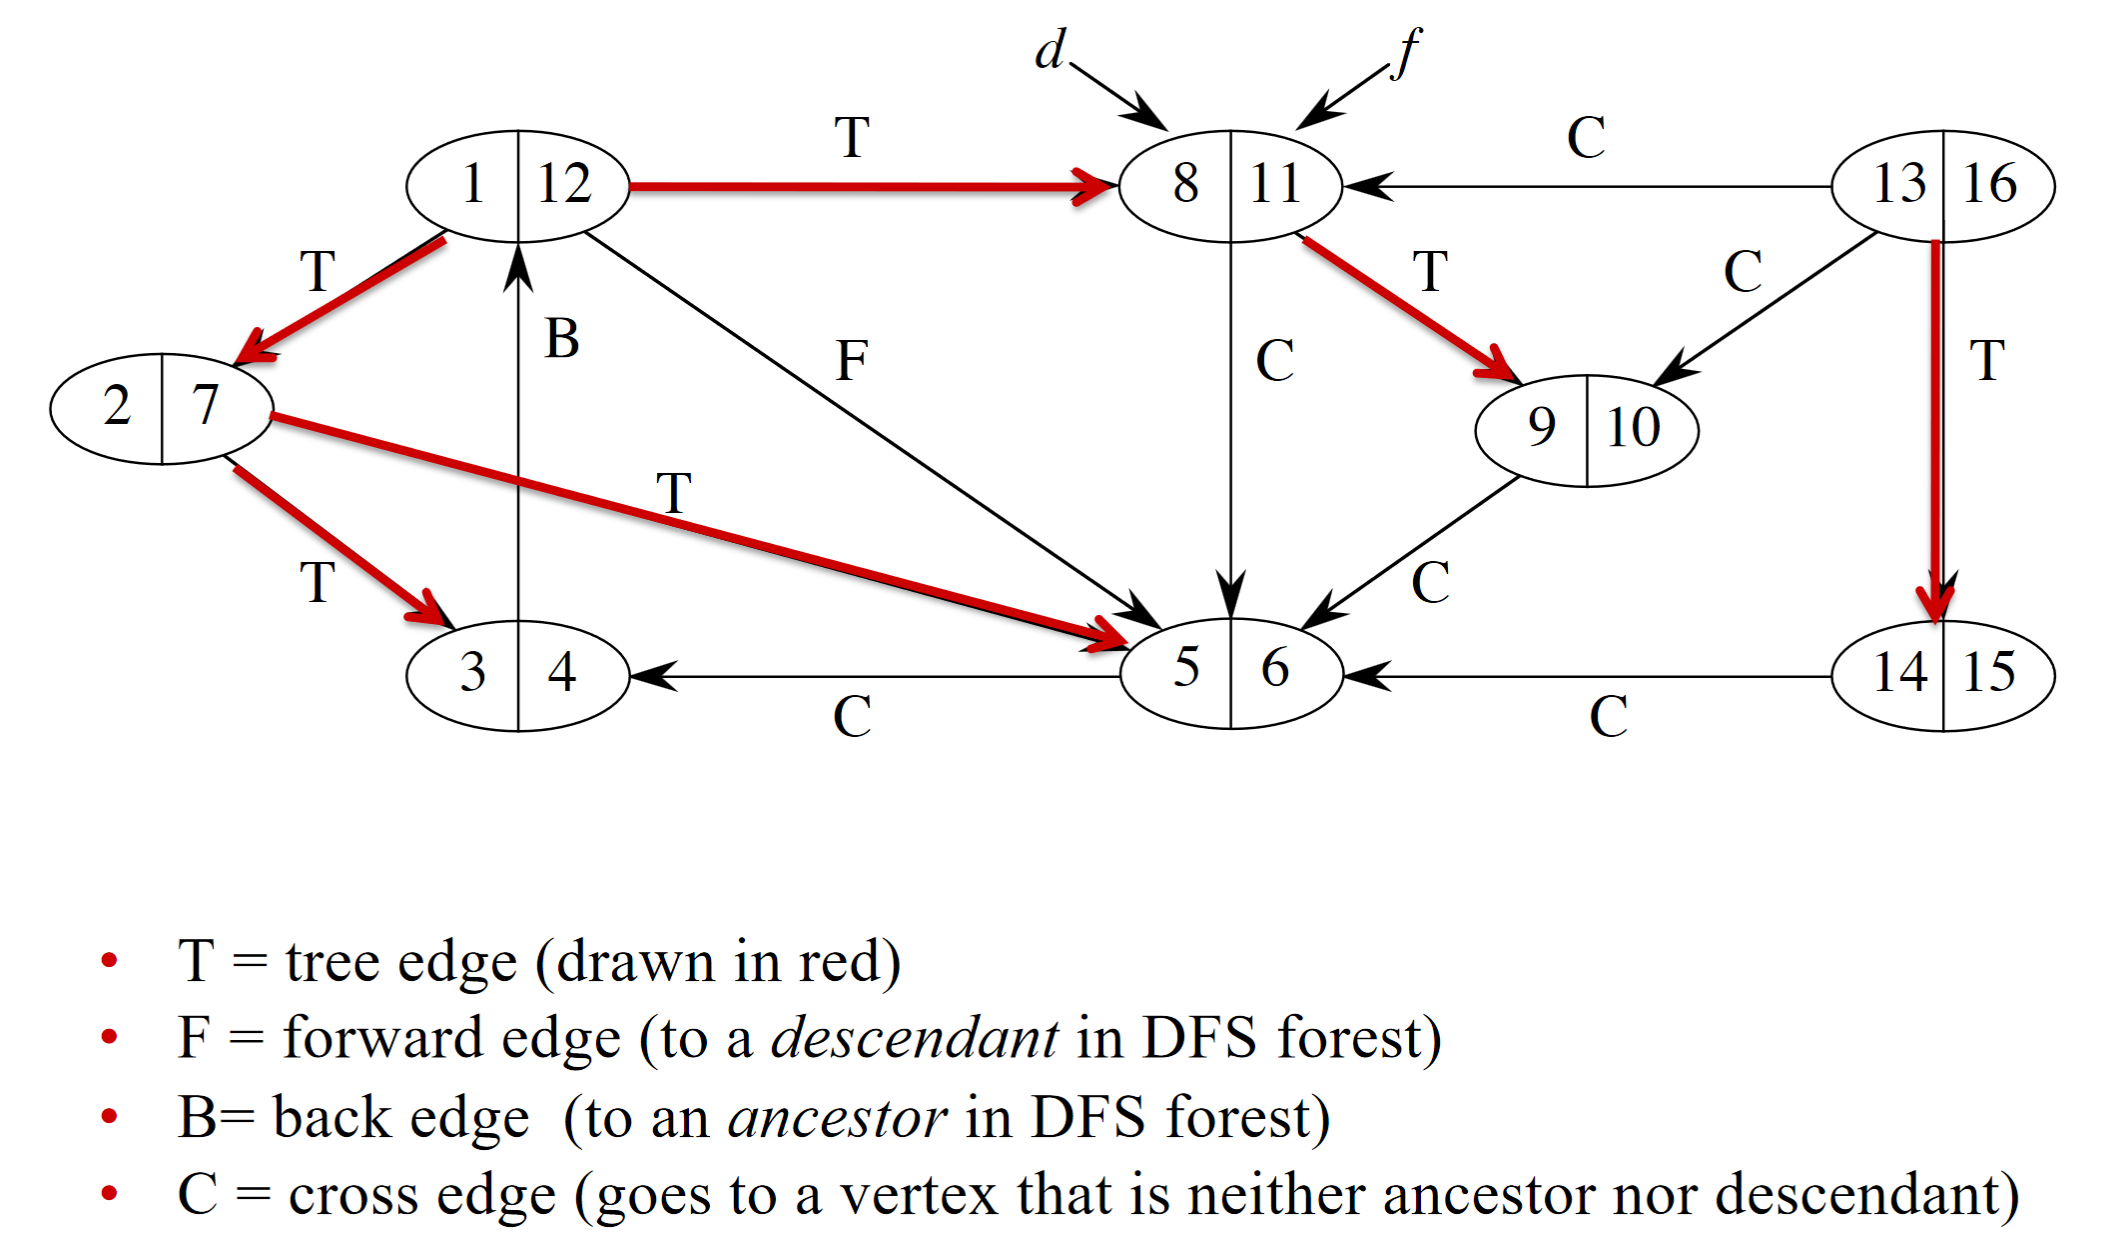
\includegraphics[height=3.5in]{./Sections/graphs/dfs.png}
%     \end{center}
%      \caption{A graph showing our $d$ discovered and $f$ finished times, denoted in pairs $(f,d)$.}\label{fig:dfs}
%   \end{figure}
    
\subsection{Edge Classifications -- Directed Graphs}

\noindent
To build our intuition around edge classifications, we'll follow a walkthrough of DFS \& BFS on directed graphs
to build our intuition. We'll follow the below format:

\begin{figure}[h]
    \begin{center}
    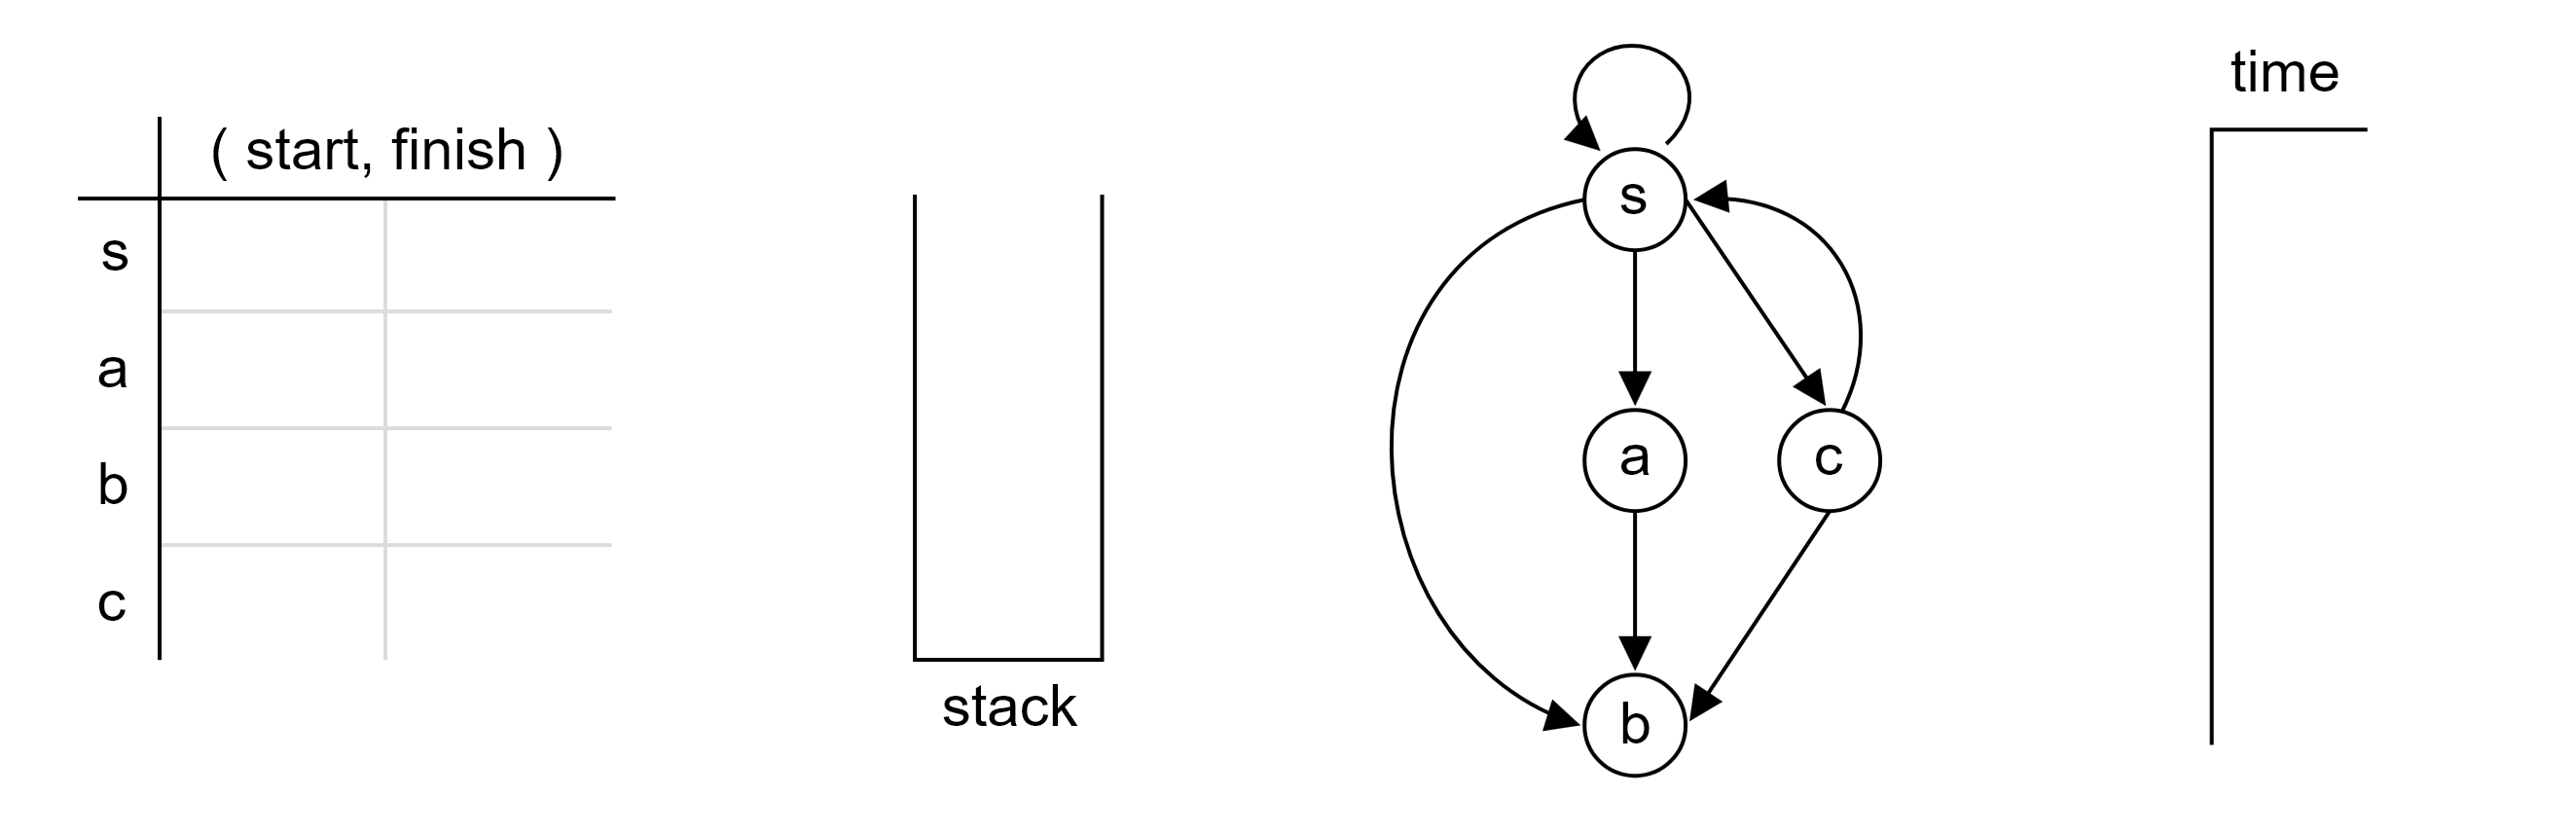
\includegraphics[width=1\textwidth]{./Sections/graphs/edges/eg_1.png}
    \end{center}
     \caption{A table for start and finish times of each visited nodes, our stack to keep track of traversals, the graph that shall be traversed, and a timer for DFS (BFS will use a queue).}
     \label{fig:edge_class}
  \end{figure}

\newpage 

\noindent
Let's start by filling out a partial DFS traversal:

\begin{figure}[h]
    \begin{center}
    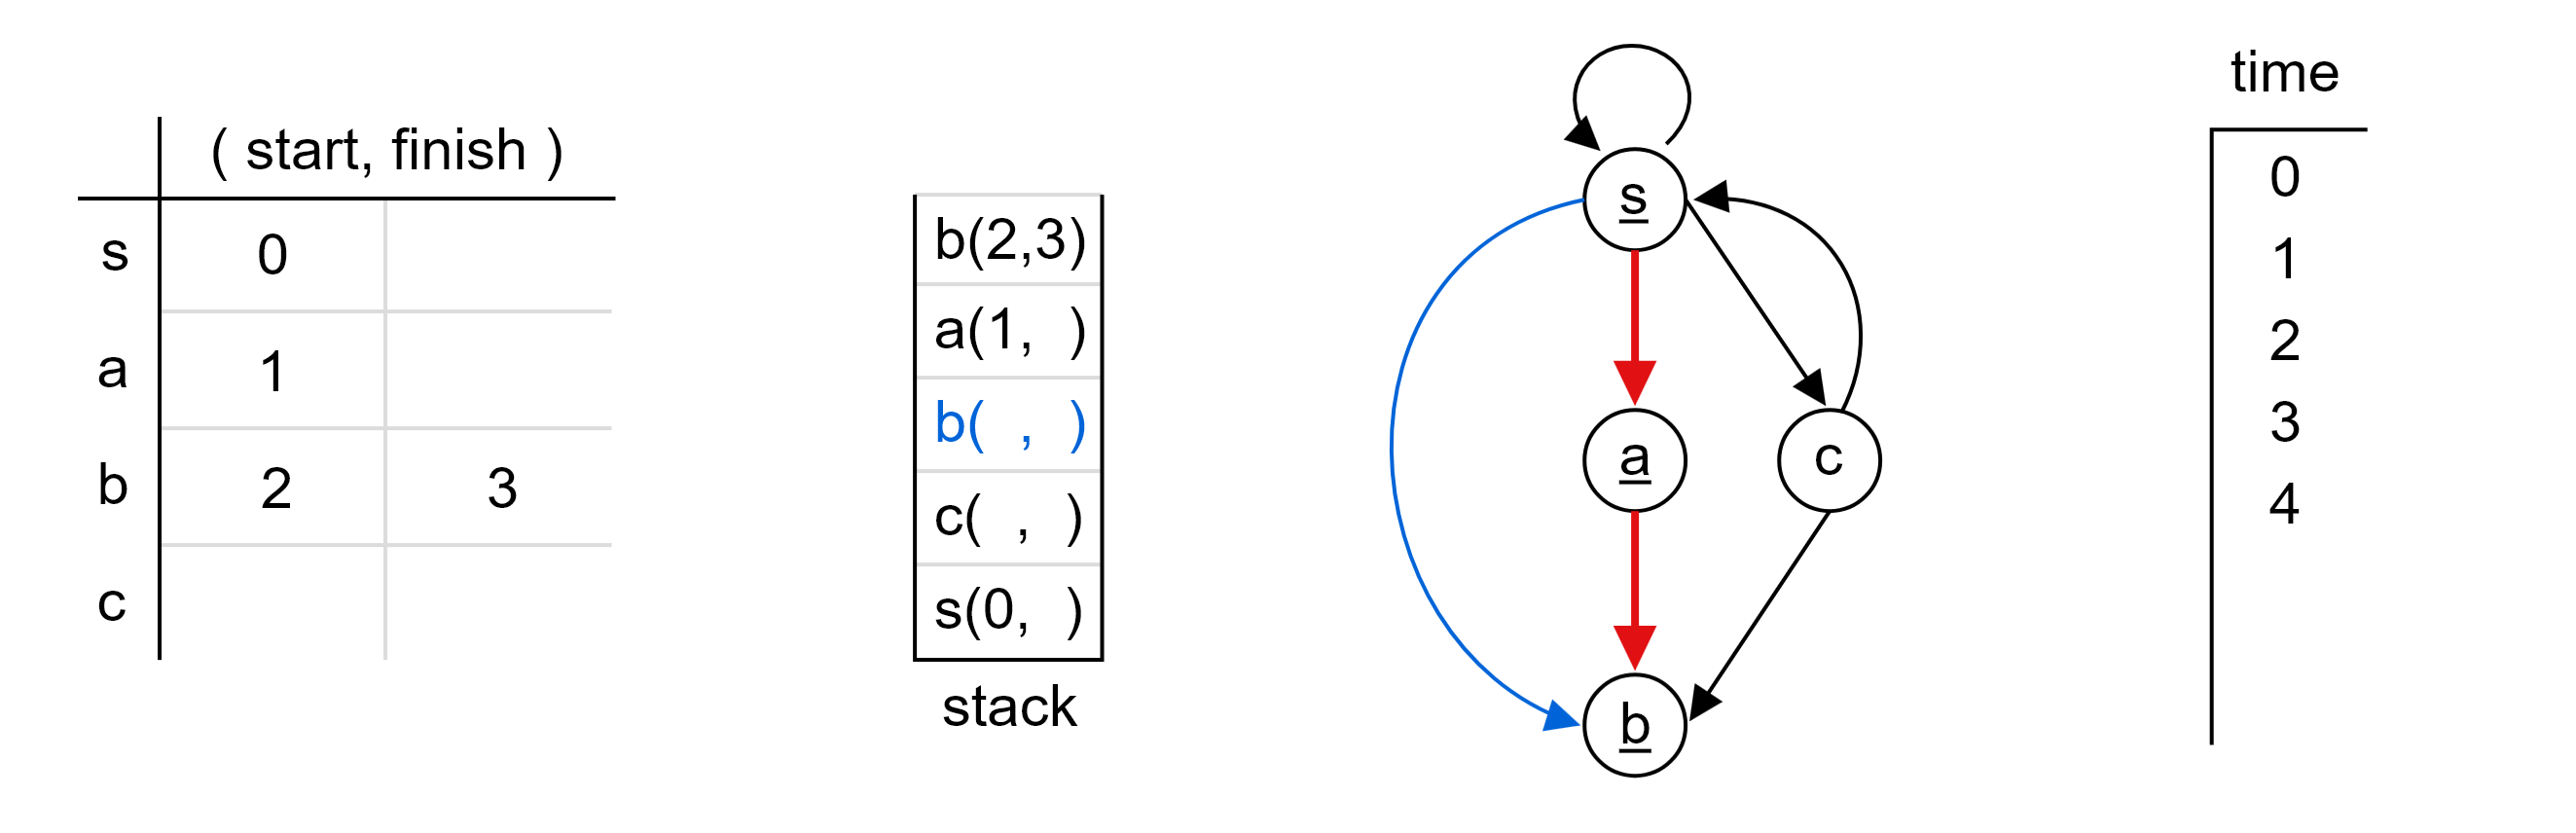
\includegraphics[width=1\textwidth]{./Sections/graphs/edges/eg_2.png}
    \end{center}
     \caption{So far we have asked $s$ to put all their children on the stack at timestamp 0. We 
     first investigate the first child $a$'s branch at time 1. It gives us $b$, for which we time stamp (2,3) for start and finish. We highlight the first the alternative $b$ branch in blue for distinction.
     The edges that are in our (start, finish) table are \underline{\textbf{Tree Edges}}.}
     \label{fig:edge_class_2}
  \end{figure}
\noindent

\begin{Def}[Forward Edge]

    A \textbf{non-tree edge} that connects an already discovered node to a descendant in the DFS tree is called a \textbf{forward edge}.
    Concretely, $(u, v)$ is a forward edge if given $u(s_1,f_1)$ and $v(s_2,f_2)$ of node id and a start finish time tuple, we have: $s_1 < s_2 < f_2 < f_1$.\\
    Where the \underline{\textbf{start time} of $u$ is less than $v$}, and the \underline{\textbf{finish time} of $u$ is greater than $v$}.
\end{Def}

\begin{figure}[h]
    \begin{center}
    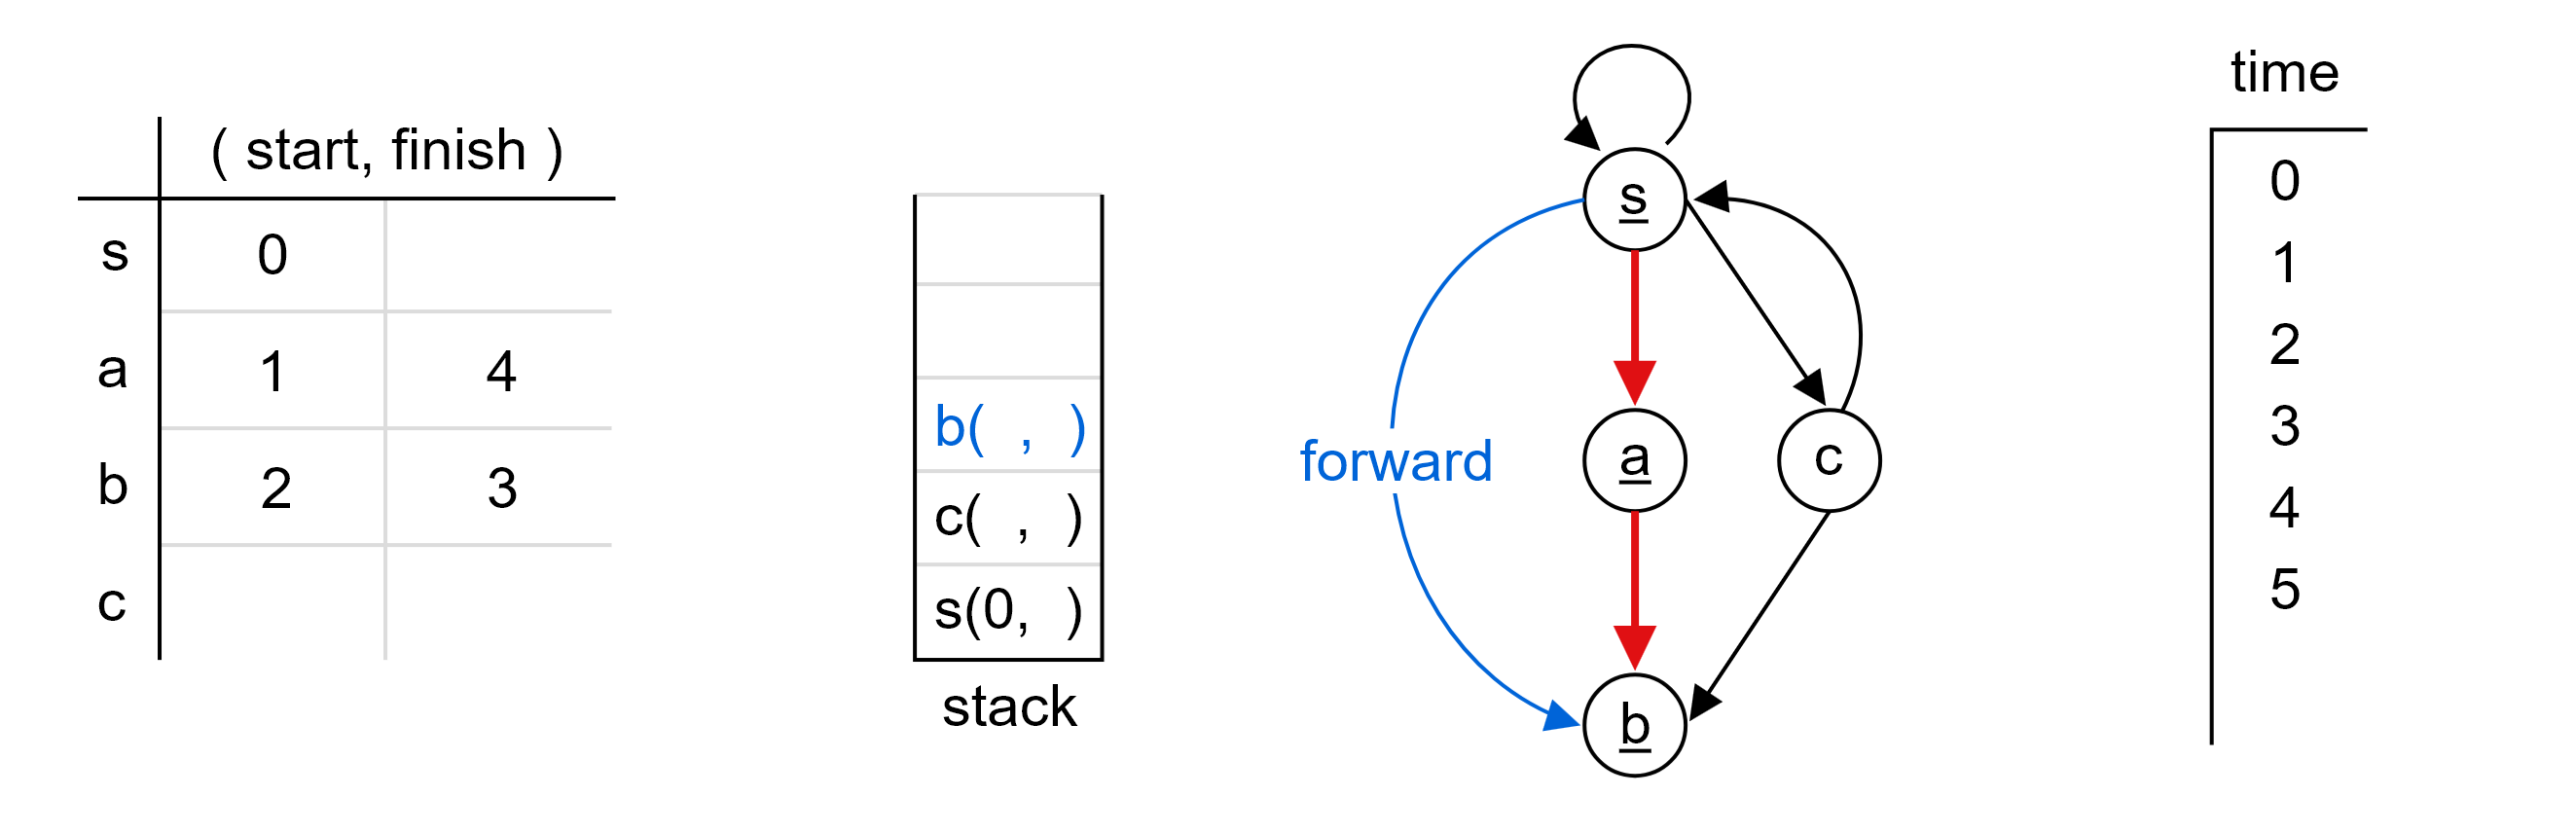
\includegraphics[width=1\textwidth]{./Sections/graphs/edges/eg_3.png}
    \end{center}
     \caption{Continuing from Figure (\ref{fig:edge_class_2}), $b$ and $a$ are taken off the stack. The next $b$ on the stack is a \textbf{forward edge}, as $s$ has a 
     smaller start time, and a foreseeable finish time than the table's $b$.}
     \label{fig:edge_class_3}
  \end{figure}

\newpage 

\noindent
The next two are \textbf{cross and back edges}:

\begin{Def}[Cross Edge]

    A \textbf{non-tree edge} that connects branches of a tree is called a \textbf{cross edge}.
    In particular, $(u, v)$ is a cross edge if $v$ is not a descendant or ancestor of $u$.
    Concretely, given $u(s_1,f_1)$ and $v(s_2,f_2)$ of node id and a start finish time tuple, we have: $s_2 < s_1 < f_2 < f_1$.\\
    Where the \underline{\textbf{start and finish time} of $u$ is greater than $v$}.
\end{Def}

\begin{Def}[Back Edge]

    A \textbf{non-tree edge} that connects a node to an ancestor in the tree is called a \textbf{back edge}.
    Concretely, given $u(s_1,f_1)$ and $v(s_2,f_2)$ of node id and a start finish time tuple, we have: $s_2 < s_1 < f_1 < f_2$.\\
    Where the \underline{\textbf{start time} of $u$ is greater than $v$}, but the \underline{\textbf{finish time} of is less than $v$}.
\end{Def}

\begin{figure}[h]
    \begin{center}
    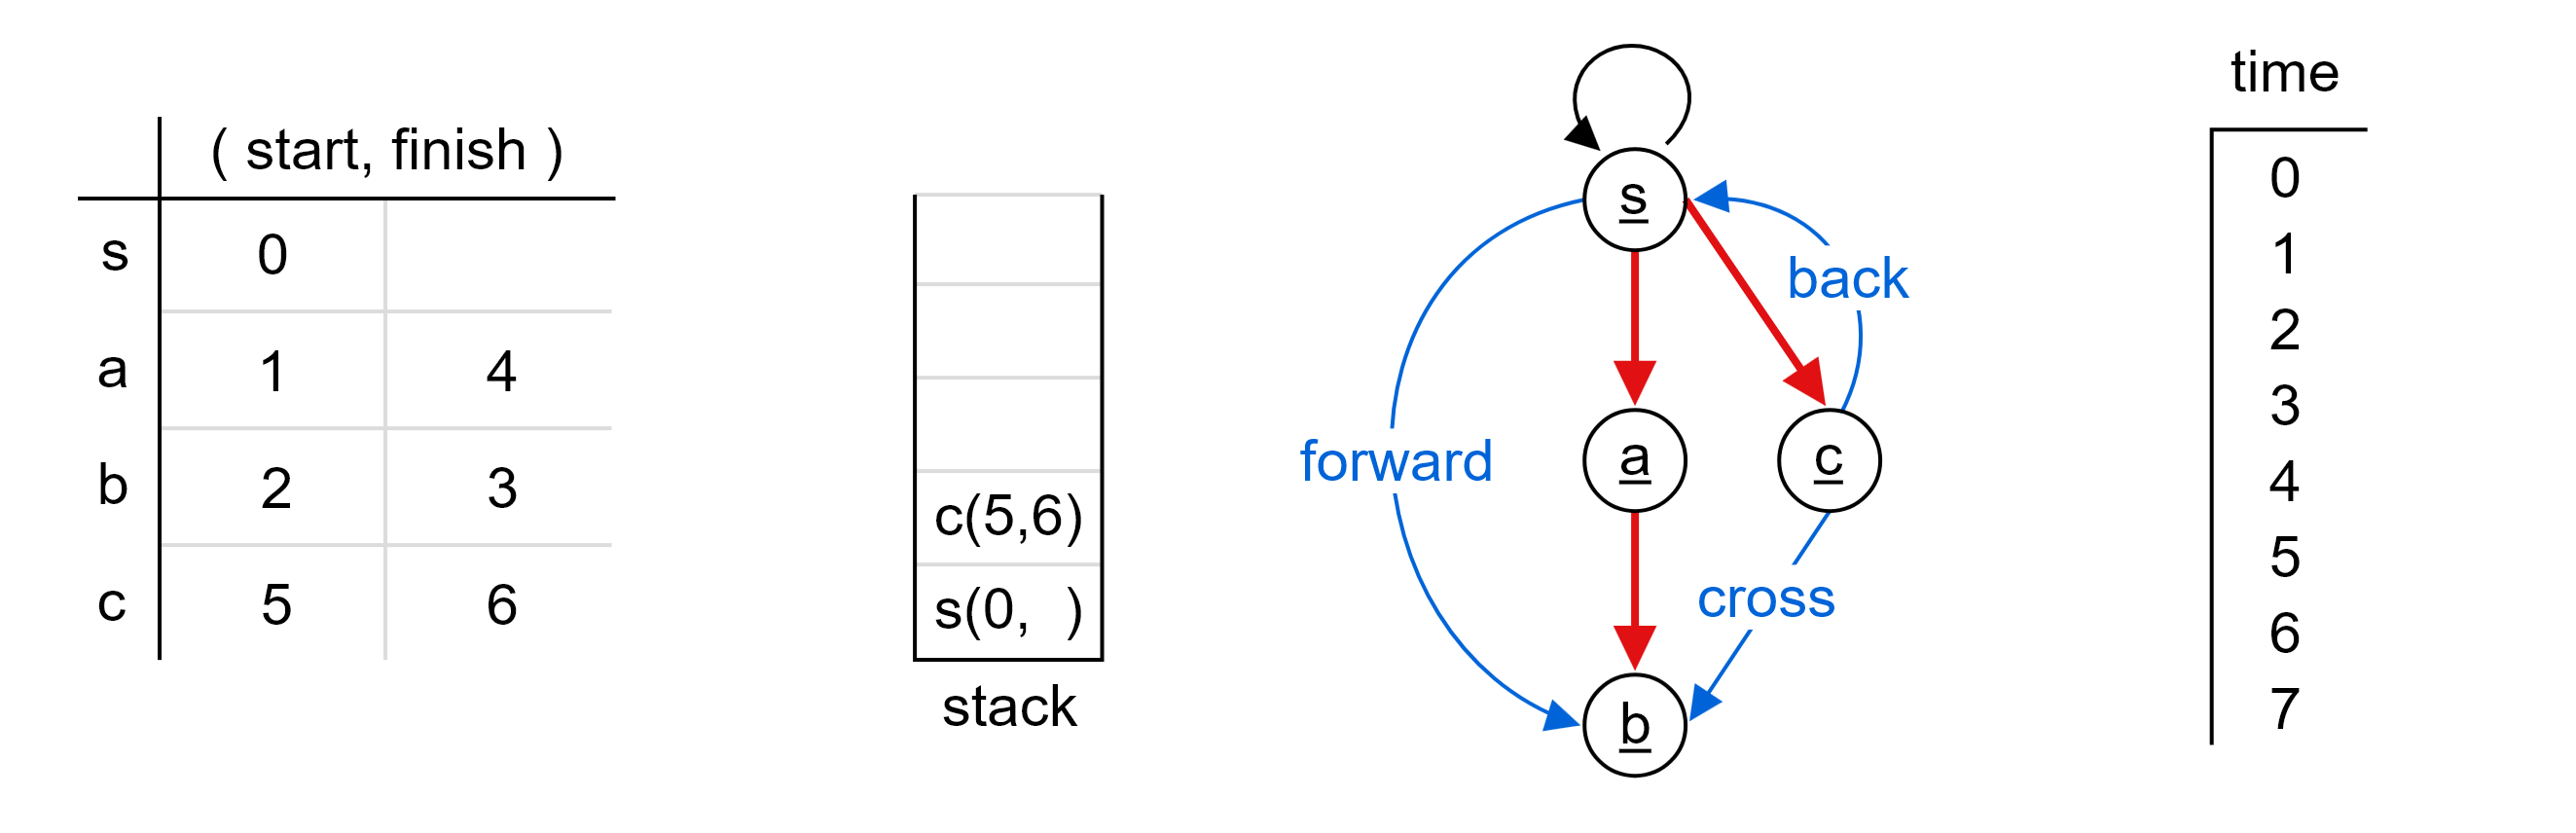
\includegraphics[width=1\textwidth]{./Sections/graphs/edges/eg_4.png}
    \end{center}
     \caption{Continuing from Figure (\ref{fig:edge_class_3}), $b$ and $a$ are taken off the stack. 
     Next on the stack is $c$, which reveals children $b$ and $s$; Here, $b$ has already been processed (cross edge), and 
     $s$ discovered, but yet to be finished (back edge). There is nothing else to explore, so we finish $c$.
     \textbf{Note:} There is no classifications for self referential edges.}
     \label{fig:edge_class_4}
  \end{figure}

\noindent
Next we'll see how our classifications work on BFS.

\newpage 

\noindent
Starting with the same graph as before we instead run BFS:

\begin{figure}[h]
    \begin{center}
    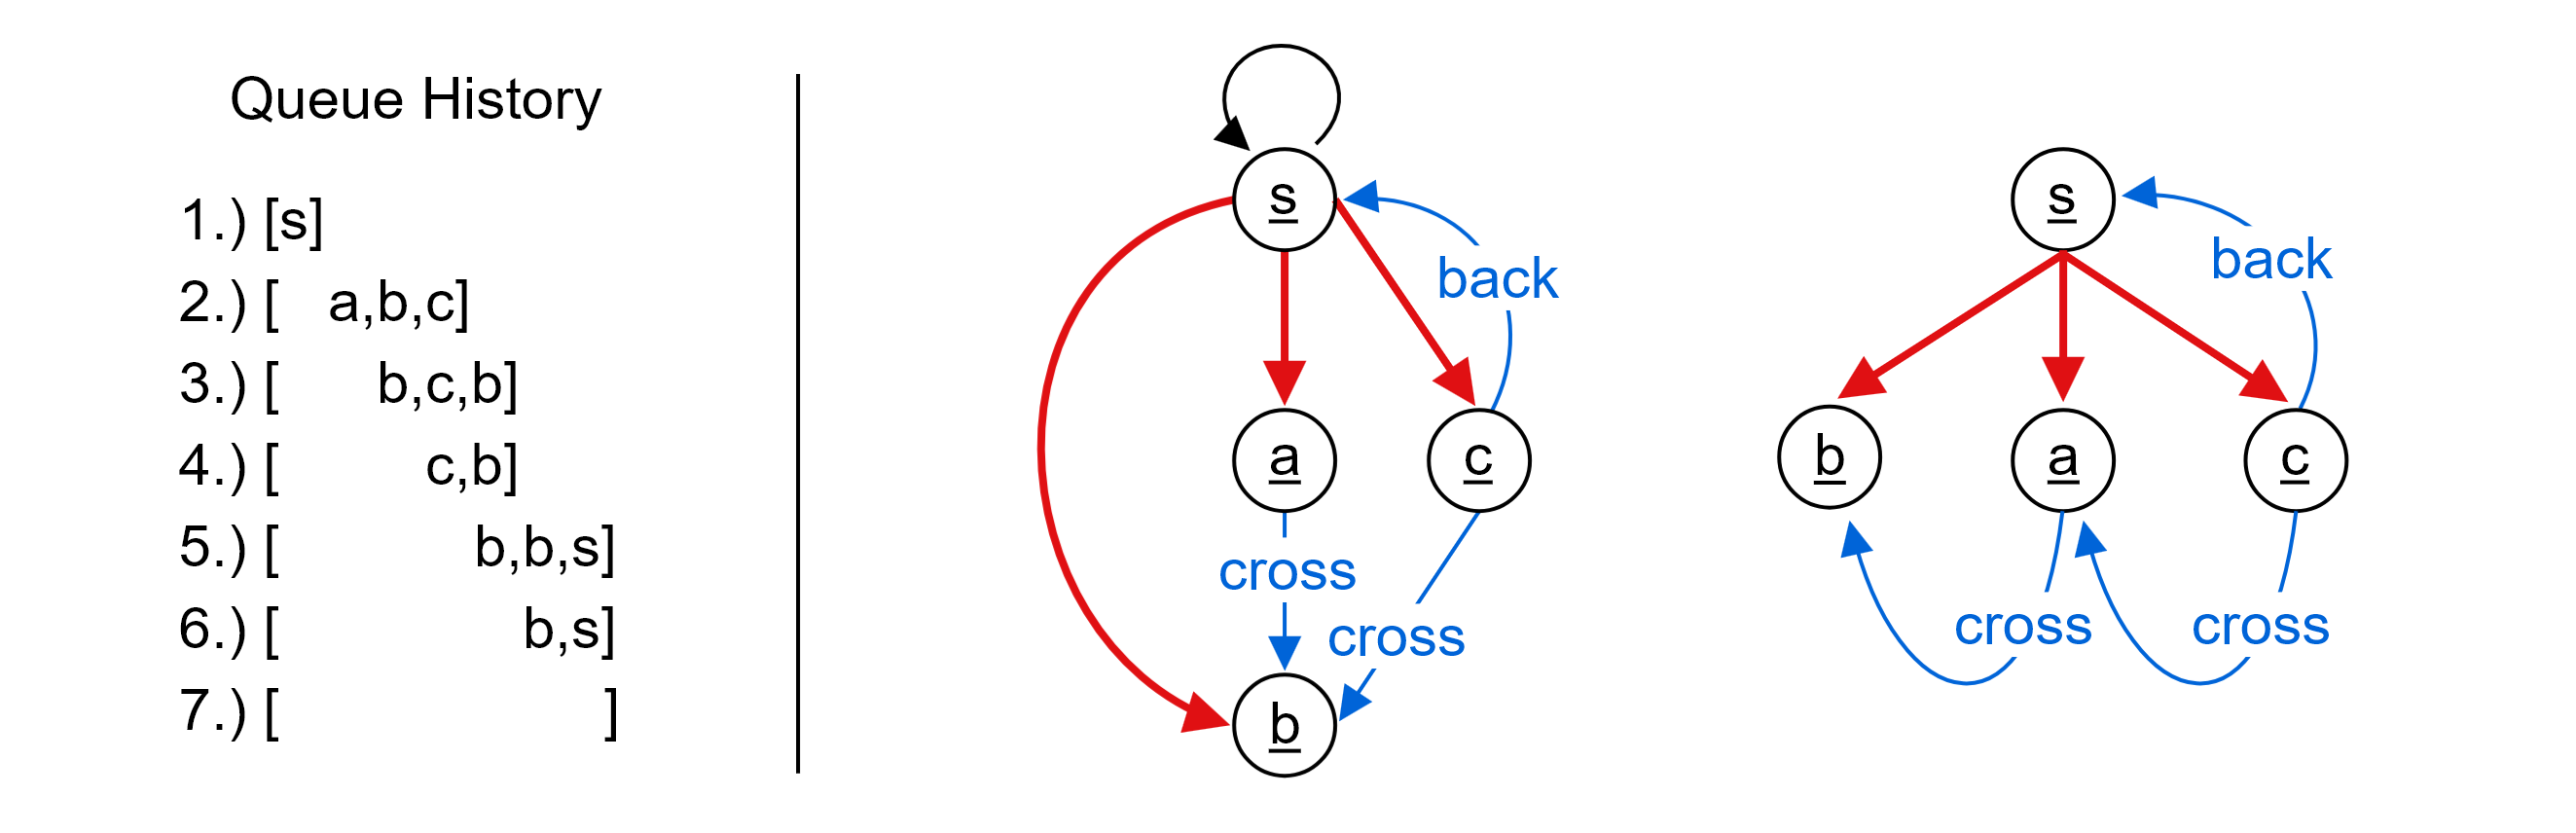
\includegraphics[width=1\textwidth]{./Sections/graphs/edges/eg_5.png}
    \end{center}
     \caption{We start with $s$ modeling the queue history on the left. The first graph is our original graph finished, and on the right it is 
     redrawn for clarity.}
     \label{fig:edge_class_5}
  \end{figure}

\begin{theo}[DFS \& BFS Directed Graphs]
    
    Between DFS and BFS, the following holds:
    \begin{itemize}
        \item \textbf{DFS}: Tree, back, forward, and cross edges (all edges).
        \item \textbf{BFS}: Tree, cross, and back edges (no forward edges).
    \end{itemize}
\end{theo}

\noindent
Additionally, one may find the following theorem helpful:
\begin{theo}[DFS and Cycles]

    Let DFS run on graph $G$, then:
    \[
\left( G \text{ has a cycle} \right) \iff \left( \text{DFS run reveals \textcolor{red}{back edges}} \right)
\]

  \end{theo}
  \begin{Proof}[Proof of Cycles and Back Edges]
    \textbf{Proving} $\left( G \text{ has a cycle} \right) \Longleftarrow \left( \text{DFS run reveals \textcolor{red}{back edges}} \right)$: Every back edge creates a cycle.\\
    \textbf{Proving} $\left( G \text{ has a cycle} \right) \Longrightarrow \left( \text{DFS run reveals \textcolor{red}{back edges}} \right)$ Suppose $G$ has a cycle:
    Let $u_1$ be the first discovered vertex in the cycle, and let $u_k$ be its predecessor in the cycle.
    $u_k$ will be discovered while exploring $u_1$.
    The edge $(u_k, u_1)$ will be a back edge.
    \end{Proof}

\newpage 

\noindent
Next we deal with undirected graphs briefly and give a summary:
\begin{figure}[h]
    \begin{center}
    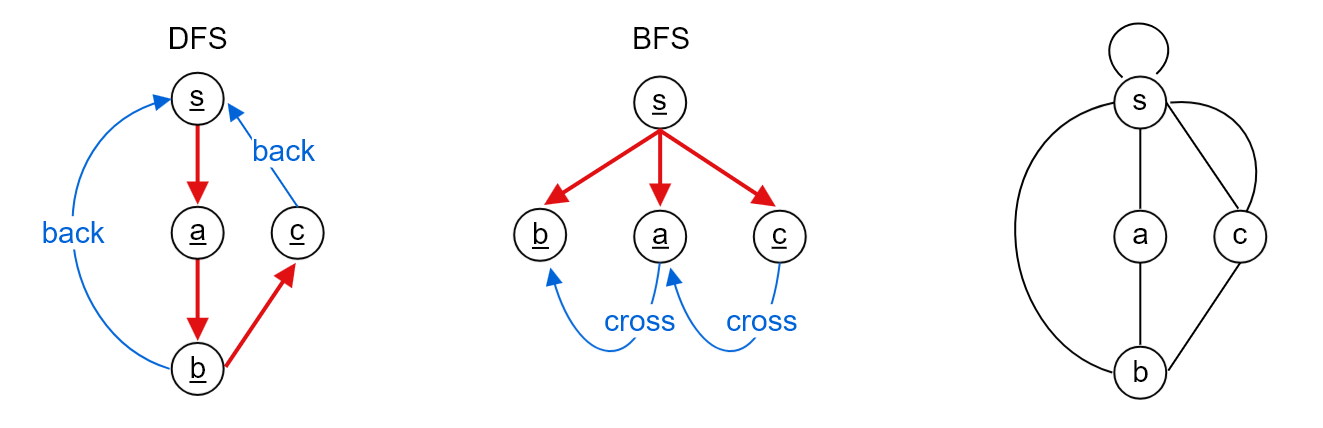
\includegraphics[width=1\textwidth]{./Sections/graphs/edges/eg_6.png}
    \end{center}
     \caption{Here DFS and BFS are shown, with the original graph on the far right. Here it's quite peculiar to have a double-edge
     in an undirected graph. In our case it's redundant and may be counted as a single edge.}
     \label{fig:edge_class_6}
  \end{figure}

  \noindent
\textbf{Summary:}\\
\noindent
This allows us to summarize the edge classifications for both directed and undirected graphs in the below table:
\begin{table}[h]
    \centering
    \begin{tabular}{|c|c|c|}
        \hline
        \textbf{Graph Type} & \textbf{DFS Edge Types} & \textbf{BFS Edge Types} \\ \hline
        Directed Graphs & Tree, Back, Forward, Cross & Tree, Back, Cross \\ \hline
        Undirected Graphs & Tree, Back & Tree, Cross \\ \hline
    \end{tabular}
    \caption{Edge classifications for DFS and BFS in directed and undirected graphs.}
    \label{tab:edge_classifications}
\end{table}

\begin{table}[h]
    \centering
    \begin{tabular}{|c|c|c|}
        \hline
        \textbf{Edge Type} & \textbf{Start Condition} & \textbf{Finish Condition} \\ \hline
        Forward Edge & less & greater \\ \hline
        Cross Edge & greater & greater \\ \hline
        Back Edge & greater & less \\ \hline
    \end{tabular}
    \caption{Summary of start and finish conditions for edge types by comparing the starting node 
    with its endpoint. E.g., in a forward edge $(u, v)$, the start time of $u$ is less than $v$, but the finish time is greater.}
    \label{tab:edge_timestamps}
\end{table}

\newpage 

\section{Binary Tree Traversals}

\noindent
First lets define a binary tree:
\begin{Def}[Binary Tree]

    A \textbf{binary tree} is a tree where each parent node has at most two children.
\end{Def}

\begin{figure}[h]
    \begin{center}
    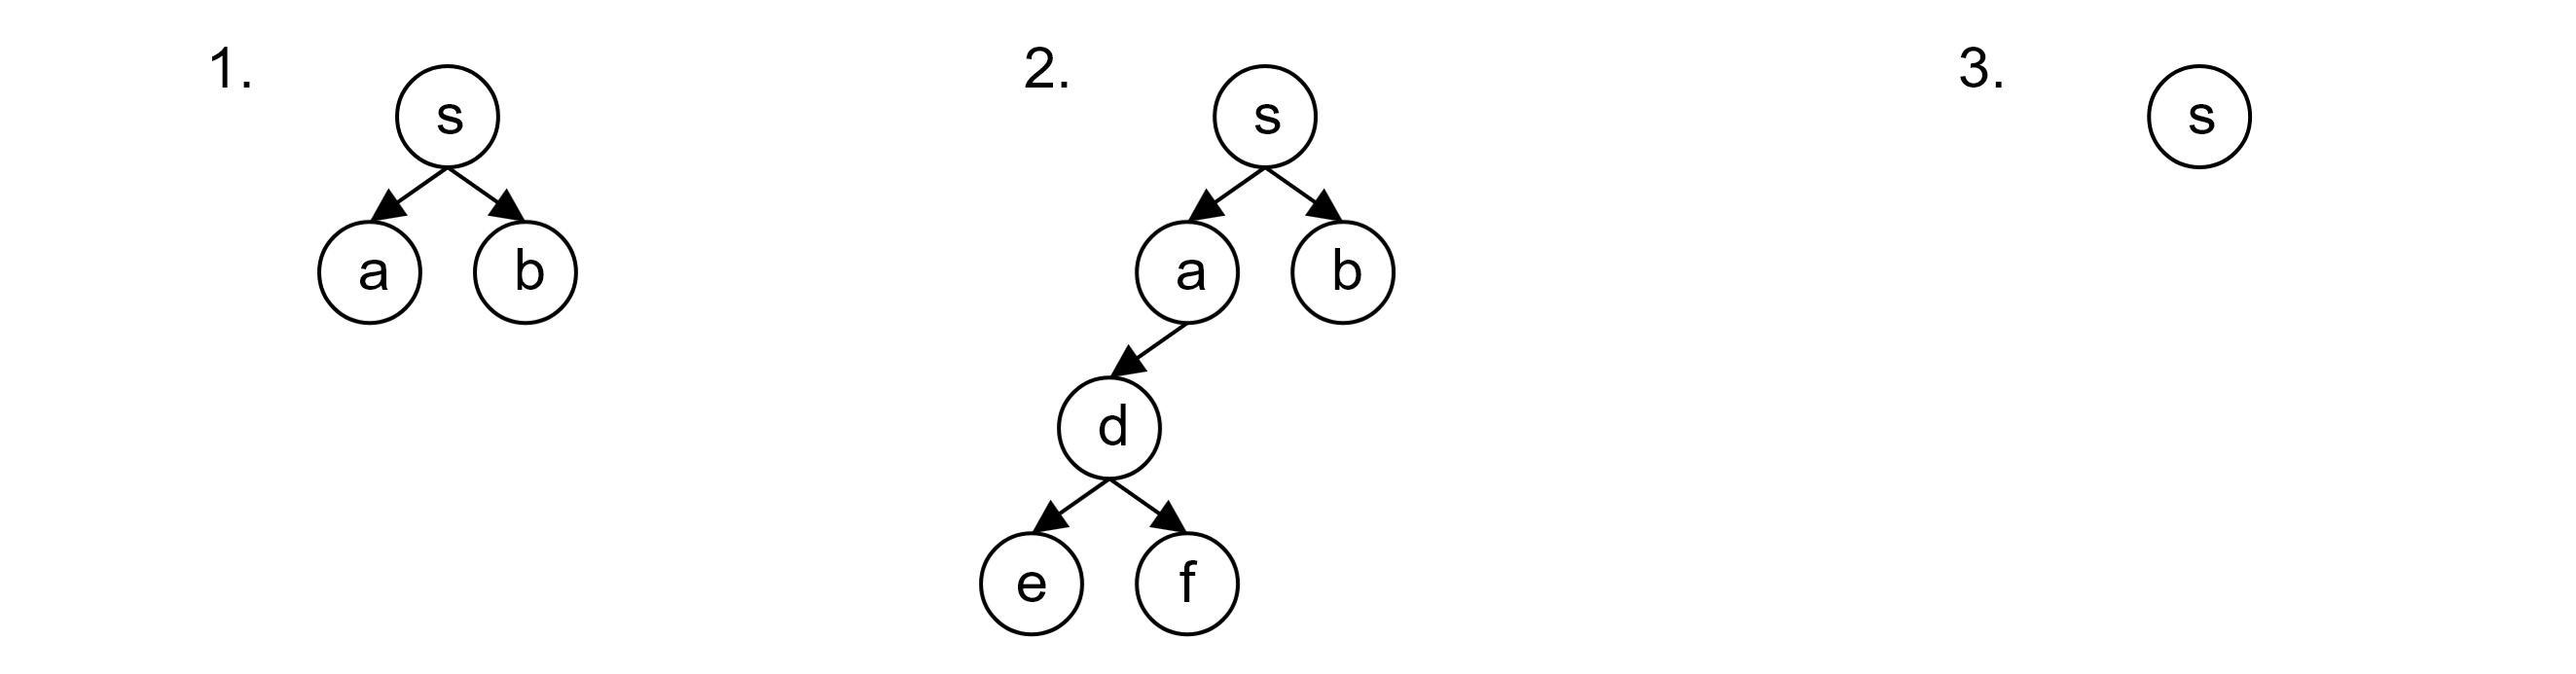
\includegraphics[width=\textwidth]{./Sections/graphs/binary_tree.png}
    \end{center}
     \caption{These are three examples of binary trees, including a single node (3).}\label{fig:binary_tree}
  \end{figure}

\noindent
To simply do a binary tree traversal, we may employ the following methods:
\begin{Func}[DFS Binary Tree Traversal - \texttt{DFS($T$)}]
    Depth-First Search on binary tree $T$ (recursive).
    
    \vspace{.5em}
    \noindent
    \textbf{Input:} Binary tree $T$.\\
    \textbf{Output:} Nodes in pre-order, in-order, and post-order.
    
    \begin{algorithm}[H]
        \SetAlgoLined
        \SetKwProg{Fn}{Function}{:}{}
        \Fn{\texttt{DFS($T$)}}{
            \If{$T$ is not empty}{
                Visit node $T$\;
                \texttt{DFS($T.left$)}\;
                \texttt{DFS($T.right$)}\;
            }
        }
    \end{algorithm}
    \noindent
    \rule{\textwidth}{0.4pt}
    \textbf{Time Complexity:} Given n nodes, and a force of a tree format, we have $n-1$ edges. Therefore with $m$ edges, $n+m = n+(n-1)$, hence $O(n)$ time.\\
    \textbf{Space Complexity:} again, we have $O(n)$ space for the stack.
\end{Func}

\noindent
$\mathbf{\rightarrow}$ \textbf{\underline{BFS has the same complexities} as per the same reasoning as the above function.}\\

\newpage
\noindent
The order in the above function is called \textbf{pre-order traversal};

\begin{Def}[Order Traversals]

    The order of traversal refers to the order in which nodes are visited/processed:
    \begin{itemize}
        \item \textbf{Pre-order:} Visit the node, then left, then right.
        \item \textbf{In-order:} Visit left, then the node, then right.
        \item \textbf{Post-order:} Visit left, then right, then the node.
    \end{itemize}
    In particular, \underline{\textbf{in-order traversal} is simply a run of \textbf{BFS}} as it processes the tree level by level starting 
    from the root.
\end{Def}

\noindent
Below is an example of all three:

\begin{Example}[Binary Tree Traversals (Part 1)]

    \begin{lstlisting}[language=Python, numbers=none]
    # Pre-order Traversal
    def PreOrder(T):
        if T is not None:
            visit(T)
            PreOrder(T.left)
            PreOrder(T.right)

    # In-order Traversal
    def InOrder(T):
        if T is not None:
            InOrder(T.left)
            visit(T)
            InOrder(T.right)

    # Post-order Traversal
    def PostOrder(T):
        if T is not None:
            PostOrder(T.left)
            PostOrder(T.right)
            visit(T)

    # Level-order Traversal
    def LevelOrder(T):
        BFS(T)
    \end{lstlisting}
\end{Example}

\newpage

\noindent
Now to show how this actually looks:
\begin{figure}[h]


    \hspace {-10em} 
\includegraphics[width=1.5\textwidth]{./Sections/graphs/binary_tree_traversals.png}
  
     \caption{%
        The above binary tree has the following traversals:\\[1em]
           $\bullet$\quad  \textbf{Pre-order:}  \hspace{.5em} G, E, C, D, A, H, K, F, M\\
           $\bullet$\quad  \textbf{In-order:}   \hspace{1.2em} C, E, A, D, G, H, F, K, M\\
           $\bullet$\quad  \textbf{Post-order:} \hspace{.05em} C, A, D, E, F, M, K, H, G\\
           $\bullet$\quad \textbf{Level-order:} G, E, H, C, D, K, A, F, M\\[1em]
         Notably, if there is no left or right child to explore for that particular traversal order, that node then and there is processed.
     For example, in in-order traversal, since $C$ has no left child, it is processed first. The same goes for Post-order, where $D$ has no right child, so it is processed.
     }\label{fig:binary_tree_traversals}
  \end{figure}
\newpage

